\chapter{Recurrences}

\section{Recurrences}

\subsection{Merge Sort}
\begin{definition}
    [Merge Sort]
    \label{def:merge_sort}
    Merge sort is a divide-and-conquer algorithm that divides a list into two halves, recursively sorts the two halves, and then merges the sorted halves.\\
    The complexity of merge sort is $T(n) = 2T\left(\frac{n}{2}\right) + O(n)$
\end{definition}

% minted python for merge sort
\begin{minted}{python}
def merge_sort(A, p, r):
    if p < r:
        q = (p + r) // 2
        merge_sort(A, p, q) # T(n/2)
        merge_sort(A, q + 1, r) # T(n/2)
        merge(A, p, q, r) # O(n)
\end{minted}

\begin{figure}
    \centering
    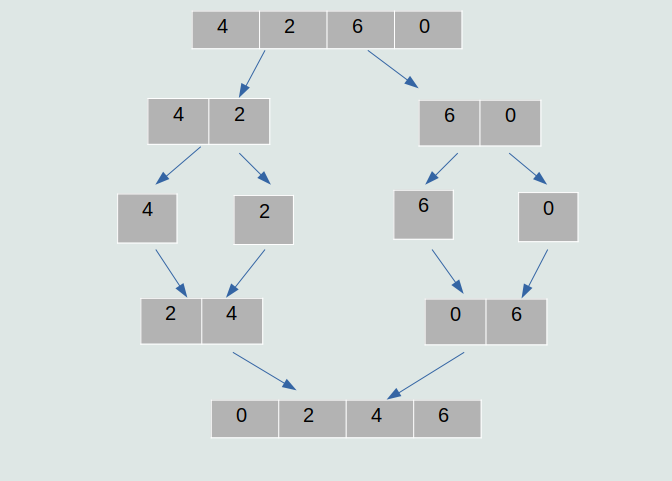
\includegraphics[width=0.5\textwidth]{./LECTURE_4/merge-sort.png}
\end{figure}

\begin{definition}
    [Master Method]
    \label{def:master_method}
    The master method is a general technique for solving recurrences of the form. \\
    Let $a \geq 1$ and $b > 1$ be constants, let $f(n)$ be a function, and let
    \[
        T(n) = aT\left(\frac{n}{b}\right) + f(n) \quad \text{has a solution}
    \]
    \begin{enumerate}
        \item If $f(n) = O(n^{\log_b a - \varepsilon})$ for some constant $\varepsilon > 0$, then $T(n) = \Theta(n^{\log_b a})$
        \item If $f(n) = \Theta(n^{\log_b a})$, then $T(n) = \Theta(n^{\log_b a} \log n)$
        \item If $f(n) = \Omega(n^{\log_b a + \varepsilon})$ for some constant $\varepsilon > 0$, and if $a f\left(\frac{n}{b}\right) \leq k f(n)$ for some constant $k < 1$ and sufficiently large $n$, then $T(n) = \Theta(f(n))$
    \end{enumerate}
    The master theorem will solve the recurrence of type $T(n) = aT\left(\frac{n}{b}\right) + f(n)$ in the case that $f(n)$ is a polynomial.
\end{definition}

\begin{example}
    Say $ a = 2, b = 2, f(n) = O(n)$, which case is this?\\
    \textbf{Solution:} This is case 2, where $f(n) = O(n^{\log_b a})$ for some constant.\\
\end{example}

\begin{example}
    $T(n) = 9T\left(\frac{n}{3}\right)$ \\
    $a = 9, b = 3, f(n) = O(n^{\log_39} = n^{2}), T(n) = \Theta(n^2)$\\
    This is case 2, where $f(n) = \Theta(n^{\log_b a})$
\end{example}

\begin{example}
    $T(n) = 3T\left(\frac{n}{4}\right) + n\log n$ \\
    $a = 3, b = 4, f(n) = n\log n, log_43 = 0.792$\\
    $f(n) = n\log n = \Omega(n^{\log_43 + \varepsilon})$ for $\varepsilon = 0.9$\\
    We got $3f(\frac{n}{4}) = 3\frac{n}{4}\log\frac{n}{4} \leq \frac{3}{4}n\log n$\\
    We pick $\varepsilon = 3/4$ so that $T(n) = \Theta(n\log n)$\\
    This is case 1, where $f(n) = O(n^{\log_b a - \varepsilon})$ for some constant $\varepsilon > 0$
\end{example}

\subsection{Substitution (Induction) Method}
\begin{remark}
    "Guess" the form of the solution and then use induction to prove it.
\end{remark}

\begin{example}
    [Substitution Method]
    \label{ex:substitution_method}
    $T(n) = 2T\left(\frac{n}{2}\right) + n$ We guess $T(n) = O(n\log n)$\\
    \textbf{Hypothesis:} Assume true for less than $n$, this is true $T(\frac{n}{2}) \leq c\frac{n}{2}\log\frac{n}{2}$\\
    \textbf{Step: }
    Due to the hypothesis, we have:
    \begin{align*}
        T(n)       & \leq 2c\frac{n}{2}\log\frac{n}{2} + n   \\
                   & = cn\log n - cn + n                     \\
                   & \leq cn\log n \quad \text{if } c \geq 1 \\
        \therefore & T(n) = O(n\log n)
    \end{align*}
    \begin{proof}
        [Eroneous Induction]
        Guess $T(n) = O(n)$. We \textbf{hypothesize} $T(\frac{n}{2}) \leq 2c\frac{n}{2}$\\
        \textbf{Step:}
        \begin{align*}
            T(n) & \leq 2c\frac{n}{2} + n \\
            \leq cn + n \leq (c + 1)n = c'n
        \end{align*}
        This is not true, as $c'$ is a completely different constant.\\
    \end{proof}
    \textbf{Basis:} \\
    $n = 1, T(1) = \leq c |\log n| = 0$ doesn't hold for $n = 1$\\
    $T(2) \leq 2 c \log 2 = 2c $ \\
    $T(4) \leq c 3 \log 3 = c3.0477$ \\
    $ \therefore \quad \text{we pick} \quad c \geq 3$
\end{example}

\begin{example}

    \begin{align*}
        T(n) & = T(\frac{n}{2}) + T(\frac{2n}{3}) + n \\
    \end{align*}
    Think of $T(n)$ as a work function, where the total work is $= hO(n)$ where $h$ is the height of the tree. \\
    \[
        \frac{2}{3}^h \times n  = 1 \iff h = \log_{\frac{3}{2}} n = O(n) \]
    total work $= O(n\log n)$
\end{example}